\subsection{Graphical User Interface}
\subsubsection{Main Window}
The User Interface is meant to provide the user with all necessary informations about the registered devices. The main window consists of two parts. 
The first part is form connecting and disconnecting the server panstamp. While attempting to establish a connection, the users can select every serial port with an attached device as well as the baut-rate. Once the Java-Server is connected, the Connect-Buttons label changes it's text and turns into a Disconnect-Button.
The second part displays a table of all the known devices, their state and a timestamp as well as their personalities name. This table updates itself with a fixed frequency, to ensure that for example every new device and/or every change in state is visible to the user.

%put picture here
\begin{figure}[h!]
 \centering
 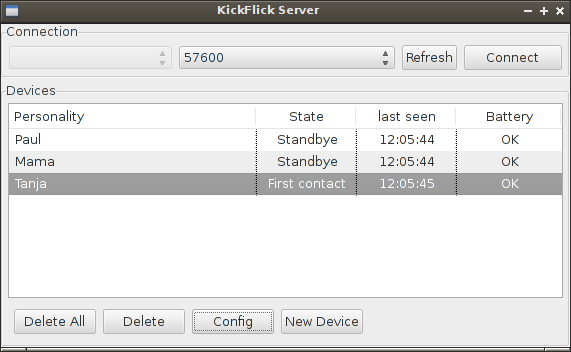
\includegraphics[width= 0.5\textwidth, clip=true  ,keepaspectratio=true]{./pic/java-server-main.png}
 % java-server-main.png: 0x0 pixel, 0dpi, nanxnan cm, bb=
 \caption{Main Window}
 \label{fig:java-server-main}
\end{figure}



If the server got at least one device, the user can select it in the device-table and open a configuration dialog by pressing either the configuration button on the bottom of the table or double clicking on the selected table item.

\subsubsection{Configuration Dialog}
Once the user decided to configure on device, this dialog opens and provides him, on three tabs, with all the necessary informations and options to configure the device and its personality full scope. %anders formulieren%

The user can decide whether he wants use a preconfigured personality for this particular device or not. No matter how the users decides, he can then begin configuring the device and personality.

On the first tab, labeled ''Basic'', the basic informations like the name of the personality, the current state and the addresses of both node. Below the users finds a table with all known action keys, and whether the device will react to this particulary key or not. The reaction willingness is hereby repressented by a checkbox showing a hock when a reaction will happen and no hock when ther will be no reaction to this key. The user can change every key value as he wishes.

%put picture here
\begin{figure}[h!]
 \centering
 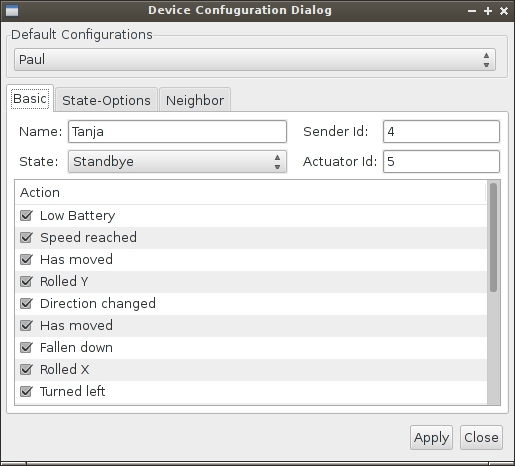
\includegraphics[width= 0.5\textwidth, clip=true  ,keepaspectratio=true]{./pic/java-server-config01.png}
 % java-server-main.png: 0x0 pixel, 0dpi, nanxnan cm, bb=
 \caption{Configuration Dialog, 1st Tab}
 \label{fig:java-server-config01}
\end{figure}

The second tab shows the seperate states a personality can reach and its color pattern and both colors for this particular state. The user can then change the pattern and the colors for every state.




% vim: spell spelllang=en_gb 
